Wir wollen unsere Werkzeuge zur Analyse von Signalen und Systemen nun um das wahrscheinlich wichtigste erweitern.
Hierbei zerlegen wir Signale, beziehungsweise Systemantworten/Impulsantworten, in ihre \q{harmonischen} Anteile -- wir transformieren in den \emph{Frequenzbereich}.
Man diese Art der \emph{Analyse} auch oft \emph{Fourier-Analyse}.
Da wir verschiedene Arten von Signalen bereits kennengelernt haben, muss diese Zerlegung auch auf verschiedene Weisen durchgef"uhrt werden.
F"ur diskrete Signale, ergibt es beispielsweise wenig Sinn, eine Integraltransformation zu definieren, Aperiodische Signale wiederum k"onnen nicht in einer Fourier-Reihe entwickelt werden, da die inh"arent der Periodizit"at widerspricht.
Das hei"st, dass f"ur jede \q{Art} von Signal und dessen Eigenschaften, die passende Transformation existiert.
Weiterhin "andert sich auch immer die \emph{Interpretation} dieser Zerlegung in harmonische Komponenten.

Dar"uber hinaus werden wir auch den umgekehrten Weg gehen.
Es ist auch m"oglich, Signale aus dem Frequenzbereich in den jeweils richtigen Definitionsbereicht zu transformieren. 
In diesem Fall spricht von von \emph{Fouriersynthese}, da wir ein Signal aus dessen Information "uber harmonische Anteile erzeugen/synthetisieren.
Wir liefern nun also die Definitionen und Zusammenh"ange der Fourier-Transformation, die wir in \Cref{sec:sampling} ohne Erl"auterungen ausgenutzt haben.

\subsection{Fourier-Transformation kontinuierlicher Signale}\label{sec:fourier:cont}

\subsubsection{Fourier-Transformation kontinuierlicher periodischer Signale}\label{sec:fourier:cont:period}

Wir haben bereits in \Cref{sec:cont_complex_harm} mit \eqref{eq:cont_fourier_series} gesehen, dass man durch Linearkombination der komplexen Sinus-Funktionen
\[
\{\exp(\jmath 2 \pi k F_0 t), \fuer k \in \Z\}
\]
eine $1/F_0=T_0$-periodische Funktion $x: \R \rightarrow \C$ durch
\[
x(t) = \Sum{k \in \Z}{}{c_k \exp(\jmath 2 \pi k F_0 t)}
\]
erh"alt.
Dies ist demnach ein Fall von \emph{Fourier-Synthese}, da wir aus den Gewichten $c_k$ in der Linearkombination eine Funktion $x$ erhalten.
Wir wollen nun den umgekehrten Weg gehen, auf welchem wir f"ur eine gegebene Funktion $x$ die Koeffizienten $c_k$ bestimmen k"onnen.
Wir starten dazu mit 
\begin{equation}\label{eq:fourier:fourier_series}
    x(t) = \Sum{k \in \Z}{}{
        c_k \exp(\jmath 2 \pi k F_0 t)
    }
\end{equation}
und multiplizieren beide Seiten mit $\exp(-\jmath 2 \pi \ell F_0 t)$ und integrieren "uber eine Periode $[0,T_0]$.
Dann erhalten wir
\[
\Int{0}{T_0}{
    x(t) \exp(-\jmath 2 \pi \ell F_0 t)
}{t} 
= \Int{0}{T_0}{
    \left(
        \Sum{k \in \Z}{}{
            c_k \exp(\jmath 2 \pi k F_0 t)
        }
    \right)
    \exp(-\jmath 2 \pi \ell F_0 t)
}{t} 
\]
und nach Vertauschung von Summation und Integration, dass
\[
\Sum{k \in \Z}{}{
    c_k 
    \Int{0}{T_0}{\exp(\jmath 2 \pi (k - \ell) F_0 t)}{t}
}
= \Sum{k \in \Z}{}{
    c_k \left[
        \frac{
            \exp(-\jmath 2 \pi (k - \ell) F_0 t)
        }{
            \jmath 2 \pi F_0(k - \ell)
        }
    \right]_{0}^{T_0}
}.
\]
Da die Funktion $\exp(-\jmath 2 \pi (k - \ell) F_0 t)$ im Fall $k \neq  \ell$ Periode $T_0$ besitzt, sind alle Summanden in der rechten Summation identisch $0$, au"ser wenn $k = \ell$.
Dann ergibt sich f"ur $\exp(\jmath 2 \pi (k - \ell) F_0 t) = 1$, also
\[
\Int{0}{T_0}{\exp(\jmath 2 \pi (k - \ell) F_0 t)}{t} 
    = \Int{0}{T_0}{1}{t} 
    = T_0.
\]
Final erhalten wir f"ur die Berechnung der Fourier-Koeffizienten $c : \N \rightarrow \C$ als Berechnungsvorschrift
\[
    c[\ell] = \frac{1}{T_0}\Int{0}{T_0}{
        x(t) \exp(-\jmath 2 \pi \ell F_0 t)
    }{t}.
\]
Wir haben in diesem Fall also \emph{Fourier-Analyse} betrieben.
Au"serdem haben wir absichtlich die Schreibweise von $c_\ell$ auf $c[\cdot]$ angepasst, um zu verdeutlichen, dass man nun die $c[\cdot]$ als \emph{komplexes diskretes Signal} auffassen k"onnen.
Dieses diskrete Signal k"onnen wir nun durch die Fourier-Reihe mit dem Signal $x : \R \rightarrow \C$ \emph{identifizieren}.
Sowohl $x$ als auch $c[\cdot]$ sind also Darstellungen desselben Sachverhaltes -- im \q{Zeitbereich} und im zugeh"origen \q{Frequenzbereich}.
Wir sehen auch, dass sich f"ur kontinuierliche und periodische Signale ein \emph{diskreter} Frequenzbereich ergibt.

Obige Herleitung verschleiert aber einen viel tiefer liegenden Zusammenhang.
Definieren wir wie in \Cref{sec:cont_complex_harm} die Funktionen $x_k : \R \rightarrow \C$ als
\[
x_k(t) = \exp(\jmath 2 \pi k F_0 t),
\]
dann k"onnen wir obige Rechnung auch so auffassen.
Wir betrachten Multiplikation von $x$ mit $x_\ell^\ast$ und anschlie"sende Integration als Skalarprodukt $\ScPr{x}{x_\ell}$. 
Au"serdem haben wir aus der Fourier-Reihe gegeben, dass
\[
x = \Sum{k \in \Z}{}{c_k x_k}
\]
Wir haben also in dieser Denkweise lediglich auf beiden Seiten der Fourierreihe in \eqref{eq:fourier:fourier_series} das Skalarprodukt mit $x_\ell$ gebildet.
Also
\[
\ScPr{x}{x_\ell} = \ScPr{\Sum{k \in \Z}{}{c_k x_k}}{x_\ell}.
\]
Das Skalarprodukt ist linear, also k"onnen wir auch
\[
\ScPr{x}{x_\ell} = \Sum{k \in \Z}{}{c_k \ScPr{x_k}{x_\ell}}
\]
schreiben.
Wir m"ussen also nur $\ScPr{x_k}{x_\ell}$ bestimmen. 
Dies haben wir aber oben schon berechnet, denn das waren die Ausdr"ucke
\[
\ScPr{x_k}{x_\ell}
    = \Int{0}{T_0}{x_k(t) x_\ell(t)^\ast}{t}
    = \Int{0}{T_0}{\exp(\jmath 2 \pi k F_0 t) \exp(-\jmath 2 \pi \ell F_0 t)}{t}
    = \Int{0}{T_0}{\exp(\jmath 2 \pi (k - \ell) F_0 t)}{t}
\]
Von oben wissen wir, dass
\[
\ScPr{x_k}{x_\ell} 
    = \left[
        \frac{
            \exp(-\jmath 2 \pi (k - \ell) F_0 t)
        }{
            \jmath 2 \pi F_0(k - \ell)
        }
    \right]_{0}^{T_0}
    = \begin{cases}
        T_0 \fuer k = \ell \\
        0, \Text{sonst.}
    \end{cases}
\]
Die $x_k$ stehen also paarweise \emph{senkrecht/orthogonal} zu einander und es gilt $\ScPr{x}{x_\ell} = T_0$.
Sie bilden ein sogenannten \emph{Orthogonalsystem}.
H"atten wir $\hat{x}_k = x_k / \sqrt{T_0}$ definiert, w"urde sogar gelten $\ScPr{\hat{x}_k}{\hat{x}_k} = 1$ und die $\hat{x}_k$ bilden eine \emph{Orthonormalsystem}.

Wenn wir nun noch einmal obige Gleichung f"ur $\ScPr{x}{x_\ell}$ betrachten, finden wir
\[
\ScPr{x}{x_\ell} 
    = \Sum{k \in \Z}{}{c_k \ScPr{x_k}{x_\ell}}
    = T_0 c_\ell,
\]
weil alle Summanden durch die Orthogonalit"at verschwinden und nur im Falle von $k = \ell$ eben $T_0$ "ubrig bleibt.
Der Fourier-Koeffzient $c_\ell$ ergibt sich also als Skalarprodukt von $x$ mit dem zugeh"origen $x_\ell$.
Es ist wichtig zu sehen, dass wir nur f"ur die Berechnung von $\ScPr{x_k}{x_\ell}$ die spezielle Form der $x_k$ eingesetzt haben und sonst nur allgemein mit den Eigenschaften von Skalarprodukten gearbeitet haben.
Das hei"st, dass man ganz allgemein Signale \q{transformieren} beziehungsweise \emph{analysieren} kann, indem man sie als Summe von paarweise orthogonalen Signalen ausdr"uckt.
Die Fourier-Reihe ist nur ein Spezialfall von diesem allgemeinen Konzept!

\begin{listing}[ht]
    \noindent
    \begin{minipage}{0.51\textwidth}
        \strut\vspace*{-\baselineskip}\newline
        \inputminted[firstline=10, lastline=44]{python3}{code/fourier_series.py}
    \end{minipage}%
    \begin{minipage}{0.48\textwidth}
        \strut\vspace*{-\baselineskip}\newline
        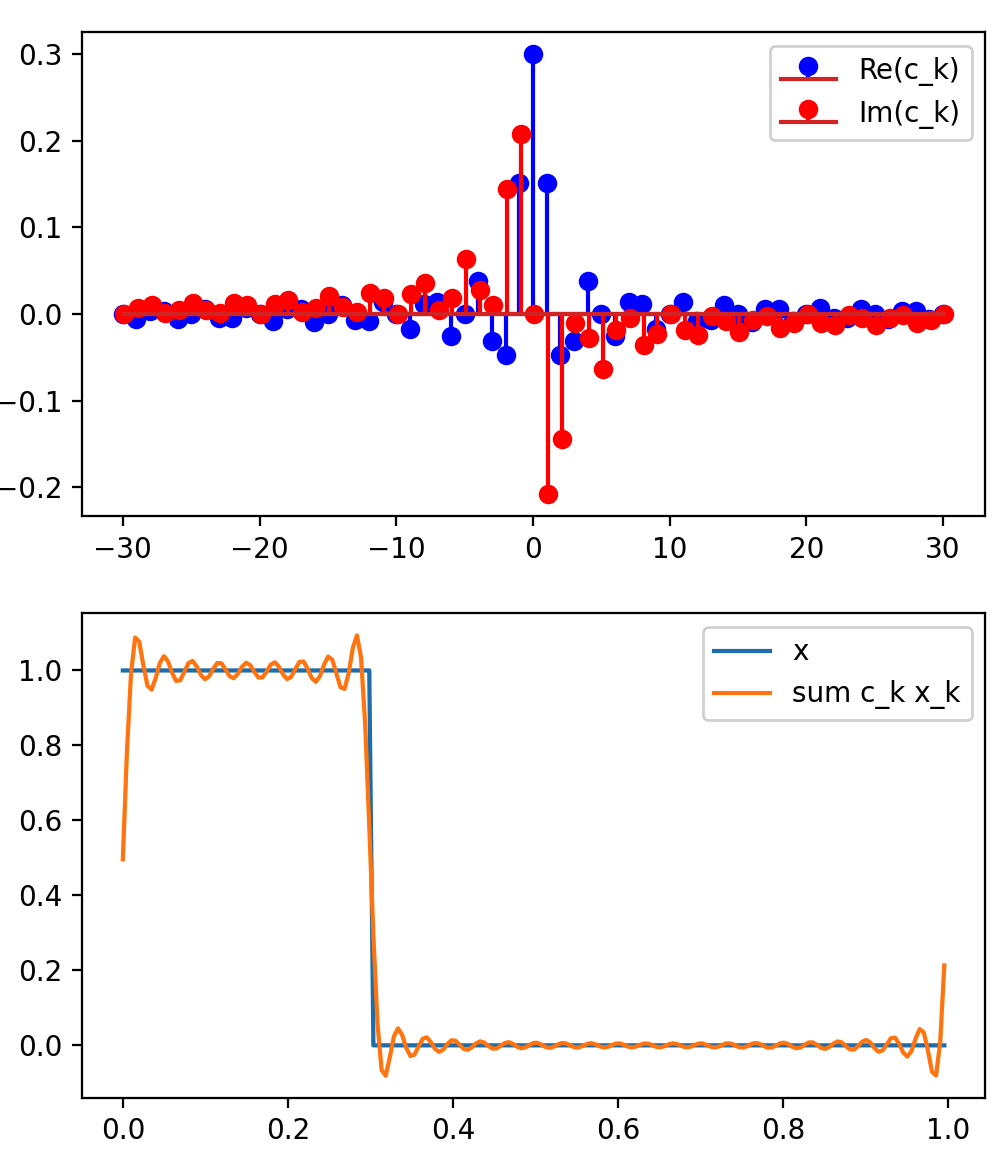
\includegraphics[width=\textwidth]{code/fourier_series.png}
    \end{minipage}
    \codecaption{dsv/code/fourier_series.py}{Berechnung und Darstellung von \eqref{eq:fourier:fourier_series}}\label{py:fourier_series}
\end{listing}
%
In \Cref{py:fourier_series} wird eine Rechteckfunktion $\Rect_{[0,T]}$ in ihre Fourier-Reihe entwickelt.
In diesem Fall m"ussen wir nat"urlich die Reihenentwicklung abbrechen, da kein $K_{\rm max}$ existiert, sodass $c[k] = 0$ f"ur $k > K_{\rm max}$.
Wir k"onnten die Reihe zwar analytisch ausrechnen, da wir jedes $x_k$ nur auf $[0,T]$ integrieren, also dem Bereich, auf dem die von uns definierte $\Rect_{[0,T]}$-Funktion Werte ungleich $0$ annimmt.
Der Einfachheit halber nutzen wir \texttt{scipy.integrate.quad}, was in der Lage ist numerische Integration relativ pr"azise durchzuf"uhren.

Es lohnt sich mit dem Wert von $K_{\rm max}$ zu experimentieren. 
Man sieht hierbei, dass gr"o"sere Werte von $K_{\rm max}$ an den Unstetigkeitsstellen $0$ und $T$ und in deren N"ahe nicht zu einer besseren "Ubereinstimmung der Fourierreiehe mit $x$ f"uhren.
Die Fourier-Reihe muss also nicht immer gegen $x$ konvergieren.
Im Falle von $\Rect_{[0,T]}$ ergibt sich das Problem genau aus dem Verhalten an $0$ und $T$ -- also Unstetigkeit, was ein generelles Problem bei der Entwicklung von Signalen in Fourier-Reihen darstellt.

Im oberen Plot von \Cref{py:fourier_series} sieht man auch, dass der Realteil der Koeffizienten $\Re{c[\cdot]}$ ein gerades diskretes Signal ist, also $c[k] = c[-k]$.
Der Imagin"arteil $\Im{c[\cdot]}$ hingegen ist ein ungerade Signal, also $c[k] = -c[-k]$\footnote{siehe \Cref{py:even_odd}}. 
Dies liegt daran, dass das Signal lediglich reelle Werte annimmt, weshalb die Symmetrie-Eigenschaften der $c[\cdot]$ allgemein f"ur reelle Signale gelten.

\begin{figure}
    \begin{center}
        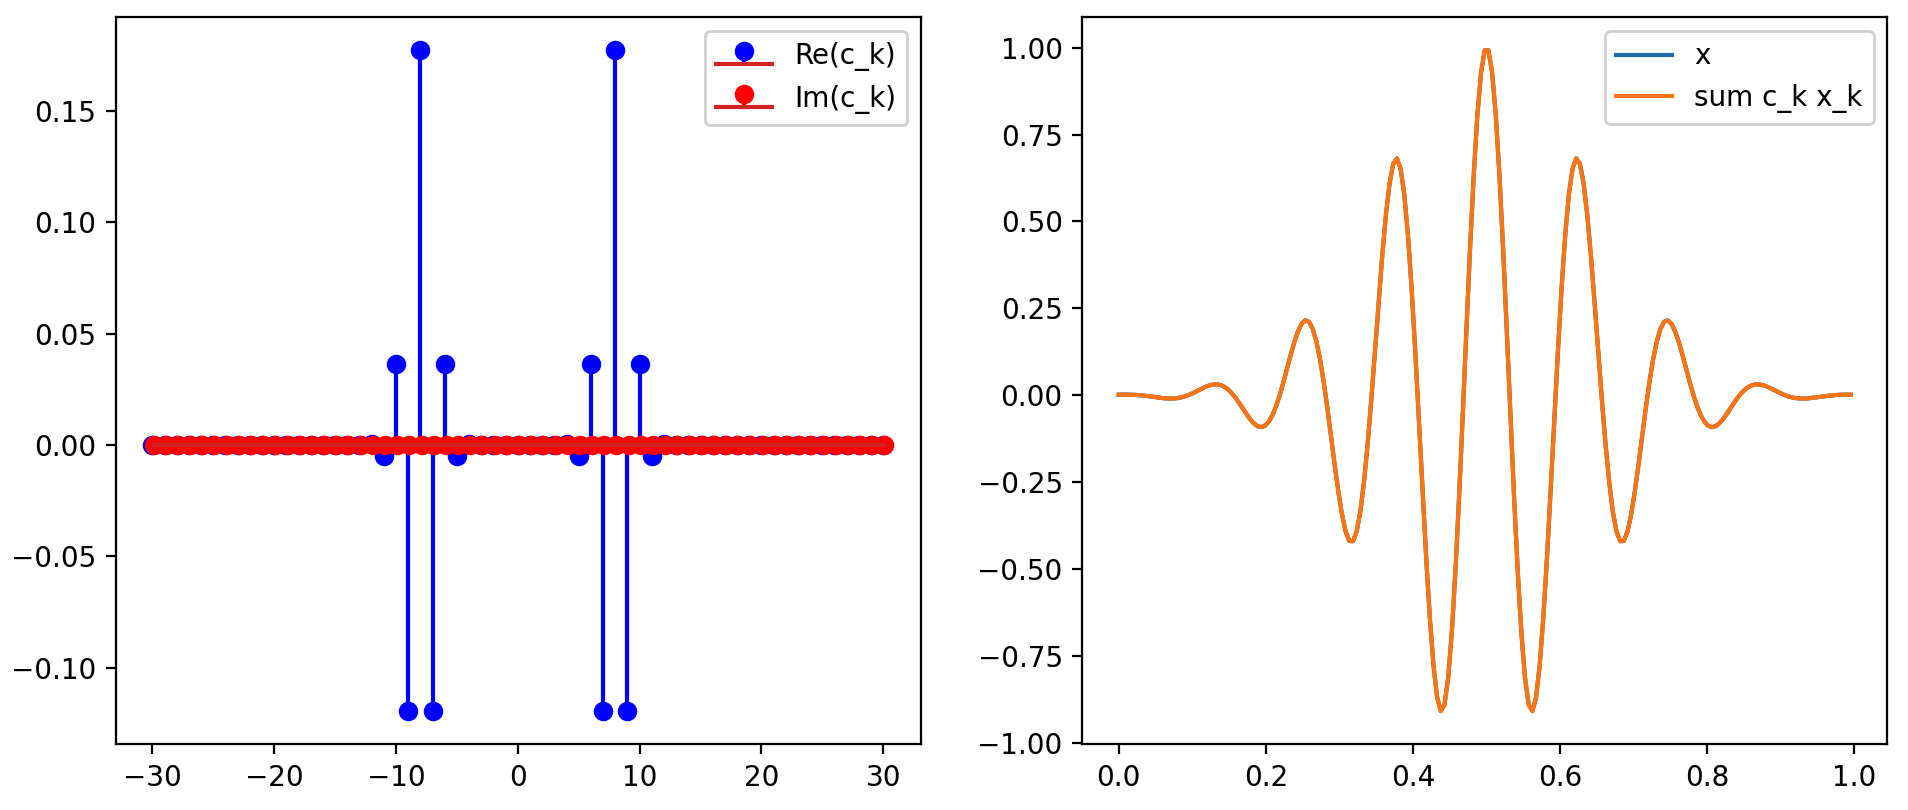
\includegraphics[width=0.8\textwidth]{code/fourier_series_1.png}

        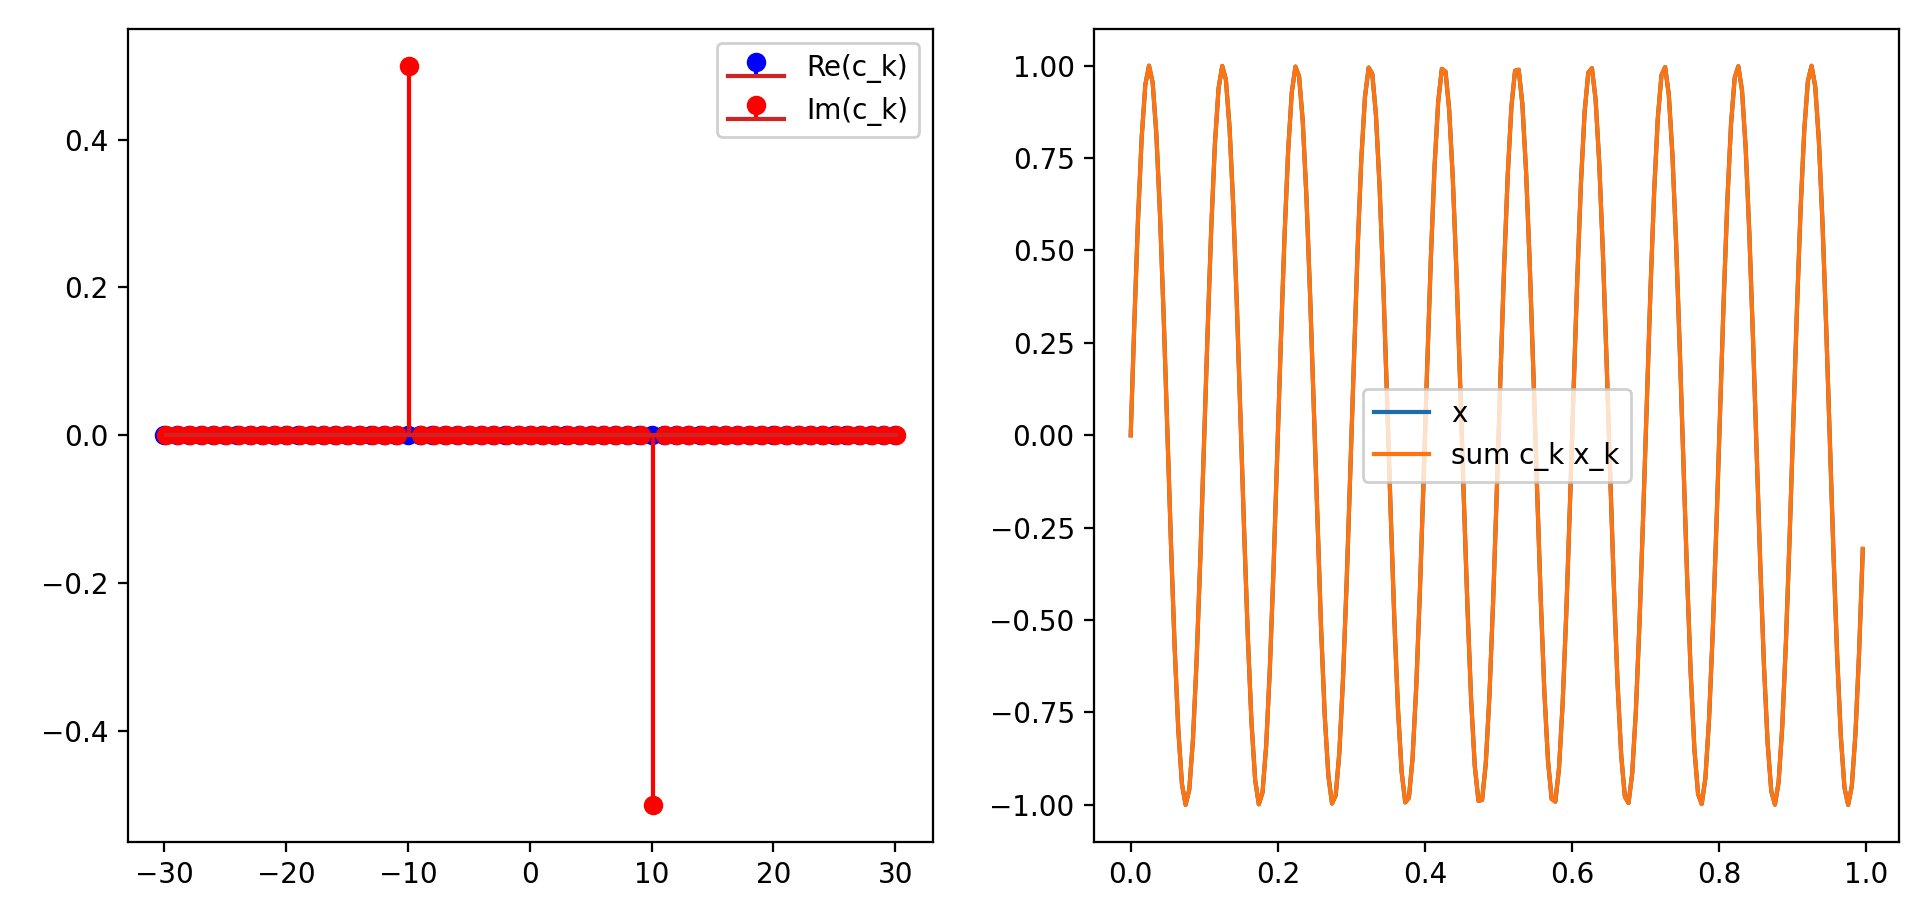
\includegraphics[width=0.8\textwidth]{code/fourier_series_2.png}
    \end{center}
    \caption{Mehr Versionen von \Cref{py:fourier_series}; Oben: $x(t) = \exp(-25(t-0.5)^2) \cos(16 \pi t)$; Unten: $x(t) = \sin(20 \pi t)$;}\label{fig:fourier:fourier_series}
\end{figure}

In \Cref{fig:fourier:fourier_series} sind noch mehr Eigenschaften der Fourier-Reihe deutlich gemacht.
Generell stellen wir fest, dass die beiden Signale jeweils gut durch eine endliche Fourier-Reihe approximiert werden k"onnen, da sie keine Unsteigkeiten aufweisen.
Im oberen Plot sieht man au"serdem, dass Achsen-Symmetrie des Signals $x$ dazu f"uhrt, dass die Imagin"arteile von $c[\cdot]$ verschwinden.
Wie man in \Cref{fig:fourier:fourier_series} unten sieht, ist es bei Anti-Symmetrie des Signals $x$ der Realteil von $c[\cdot]$, der verschwindet.
Dies liegt daran, dass der Realteil der $x_k$ eine gerade Funktion ist und der Imagin"arteil respektive eine ungerade Funktion.
Da wir in \Cref{py:even_odd} schon gesehen haben, dass ungerade und gerade Anteile eines Signals im Sinne von Skalarprodukten orthogonal sind, gilt dies auch f"ur die resultierenden Fourier-Koeffizienten.
In \Cref{fig:fourier:fourier_series} unten sieht man auch, dass man f"ur gewisse Signale die Fourier-Reihe direkt angeben kann.
Im Falle des Beispiels gilt n"amlich
\[
x(t) 
    = \sin(10 \cdot 2 \pi t) 
    = \frac{1}{2 \jmath} \left(
        \exp(10 \cdot 2 \pi t) - \exp(-10 \cdot 2 \pi t)
    \right) 
    = \frac{1}{2 \jmath} x_{10} - \frac{1}{2 \jmath} x_{-10}.
\]
Das hei"st, dass wir $x$ \emph{direkt} in seine Fourier-Reihe entwickelt haben, da wir es als Linearkombination der $x_k$ dargestellt haben.
Das hei"st es sind nur $x_{10}$ und $x_{-10}$ notwendig, um $x$ darzustellen und beide Koeffizienten haben ausschlie"slich imagin"are Anteile.

"Ahnlich wie bei der $z$-Transformation kann man also an der Fourier-Reihe Eigenschaften des Signals $x$ direkt ablesen, oder umgekehrt von Eigenschaften des Signals $x$ auf Eigenschaften der Fourier-Koeffizienten $c[\cdot]$ schlie"sen.
Au"serdem werden wir f"ur die noch folgenden Versionen der \gls{ft} sehr analoge Zusammenh"ange finden.

\subsubsection{Leichtungsdichte-Spektrum periodischer Signale}

Das Leichtungsdichtespektrum eines $T_0$-periodischen Signals $x: \R \rightarrow \C$ is gegeben durch
\begin{equation}\label{eq:fourier:period_psd}
P(x) = \frac{1}{T_0}\Int{0}{T_0}{\Abs{x(t)}^2}{t}
     = \frac{1}{T_0}\Int{0}{T_0}{x(t) x(t)^\ast}{t}
     = \frac{1}{T_0} \ScPr{x}{x}.
\end{equation}
Wir wollen nun $P(x)$ in Abh"angigkeit der Fourier-Koeffizienten $c[\cdot]$ berechnen.
Wir entwickeln also
\[
x(t) = \Sum{k \in \Z}{}{
    c_k \exp(\jmath 2 \pi k F_0 t)
}
\]
und setzen dies in $P$ ein, um
%
\begin{equation}\label{eq:fourier:series_parseval}
    \frac{1}{T_0}\Int{0}{T_0}{x(t) x(t)^\ast}{t}
        = \frac{1}{T_0}\Int{0}{T_0}{
            x(t) 
            \Sum{k \in \Z}{}{
                c_k^\ast \exp(-\jmath 2 \pi k F_0 t)
            }
        }{t}
        = \Sum{k \in \Z}{}{
            c_k^\ast 
            \frac{1}{T_0}\Int{0}{T_0}{
                x(t)
                \exp(-\jmath 2 \pi k F_0 t)
            }{t}
        }
        = \Sum{k \in \Z}{}{
            c_k^\ast c_k
        }
\end{equation}
%
als den \emph{Satz von Parseval}\footnote{\url{https://de.wikipedia.org/wiki/Satz\_von\_Parseval}} zu erhalten.
Die physikalische Interpretation ist, dass $\Abs{c[k]}$ der Leistung des Signals bei der Frequenz $k F_0$ entspricht.
Jeder Index $k$ hat also eine physikalische Gr"o"se, die mit ihm assoziiert ist.

Da nur die Frequenzen $k F_0$ f"ur $k \in \Z$ auftreten, also Frequenzen wie $0.1 F_0$ nicht vorhanden sind, sprechen wir von einem \emph{diskreten Spektrum}.
Es ergibt sich also direkt folgender wichtiger Zusammenhang: Periodische Signale im Zeitbereich besitzen ein \emph{diskretes} Spektrum.
Andersherum ergibt sich auch: Signale mit diskretem Spektrum sind periodisch.
Beide Argument ergeben sich aus der Fourier-Reihe.
Damit haben wir das duale Ergebnis zu \eqref{eq:spectrum_sampled} gefunden.
Dort f"uhrte Diskretisierung im Zeitbereich, also Sampling/Abtastung, zu einer Periodifizierung im Frequenzbereich.

\begin{listing}[ht]
    \noindent
    \begin{minipage}{0.51\textwidth}
        \strut\vspace*{-\baselineskip}\newline
        \inputminted[firstline=5, lastline=14]{python3}{code/period_psd.py}
    \end{minipage}%
    \begin{minipage}{0.48\textwidth}
        \strut\vspace*{-\baselineskip}\newline
        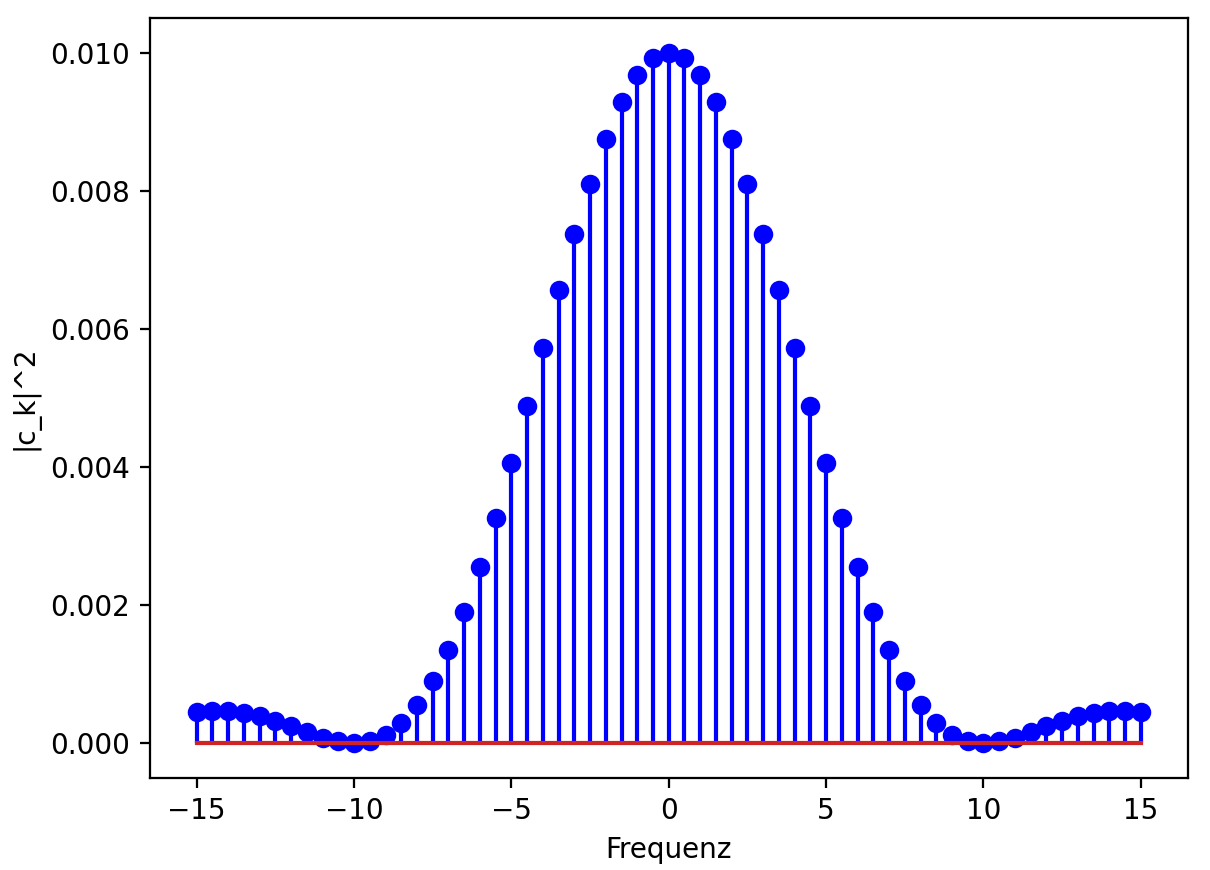
\includegraphics[width=\textwidth]{code/period_psd.png}
    \end{minipage}
    \codecaption{dsv/code/period_psd.py}{Modizifiertes \Cref{py:fourier_series} und Plot von $P$ im Frequenzbereich.}\label{py:period_psd}
\end{listing}

In \Cref{py:period_psd} zeigen wir eine Modifikation von \Cref{py:fourier_series}, in welcher wir $T_0 = 2$ setzen, also $F_0=1/2$ erhalten. 
Auf der Frequenzachse sehen wir, dass demnach diese f"ur $K_{\rm max} = 30$ also von $-15$ bis $+15$ reicht.
%
%
\FloatBarrier
\subsubsection{Fourier-Transformation von kontinuierlichen aperiodischen Signalen}
%
Um die Einschr"ankung auf periodische Signale zu vermeiden, nutzen wir die \acrlong{ft}, wie wir sie bereits in \eqref{eq:sampling:fourier_trafo} f"ur ein Signal $x : \R \rightarrow \C$ durch
\begin{equation}\label{eq:fourier:fourier_trafo}
    X(F) = \Int{-\infty}{+\infty}{x(t) \exp(-\jmath 2 \pi F t)}{t}
\end{equation}
definiert haben.
Im Unterschied zu \eqref{eq:fourier:fourier_series} integrieren wir nun "uber ganz $\R$, da sich das Signal nicht mehr periodisch wiederholt.
Aus diesem Grund ergibt sich auch ein \emph{kontinuierliches} Spektrum, da wir uns nicht mehr auf eine abz"ahlbare Menge von diskreten Frequenzen zur"uckziehen k"onnen.
Deshalb ergibt sich auch f"ur die Synthese des Signals, dass wir auch in diesem Fall integrieren anstatt summieren m"ussen, es gilt also
\begin{equation}\label{eq:fourier:inv_fourier_trafo}
    x(t) = \Int{-\infty}{+\infty}{X(F) \exp(\jmath 2 \pi F t)}{F}.
\end{equation}
Da sich f"ur die meisten Signale, die wir betrachten werden, Integration und Summation \q{"ahnlich} verhalten, finden wir auch die obigen Eigenschaften bez"uglich Symmetrien, etc., von \eqref{eq:fourier:fourier_series} wieder.

Es gibt aber eine Verbindung zur Fourier-Reihe, die wir im Folgenden kurz erl"autern wollen.
Nehmen wir an, es existiert ein $T > 0$, sodass $\Abs{x(t)} = 0$ f"ur alle $t$ mit $\Abs{t} > T$.
Dann k"onnen wir das Signal $x$ periodifizieren mit Periode $T$, indem wir
\[
x_p(t) = \Sum{k \in Z}{}{x(t - 2kT)}
\]
setzen.
Dies haben wir bereits in "ahnlicher Form in \eqref{eq:spectrum_sampled} gesehen. 
Dort hat es sich aber aus Berechnungen ergeben und hier \emph{setzen} wir diesen Zusammenhang explizit.
Dann k"onnen wir $x_p$ in seine Fourier-Reihe 
\[
x_p(t) = \Sum{k \in \Z}{}{c_k \exp(\jmath 2 \pi k t/T)}
\Text{mit}
T\,c_k = \Int{-T/2}{+T/2}{x_p(t) \exp(- \jmath 2 \pi k t/T)}{t}
    = \Int{-\infty}{+\infty}{x(t) \exp(- \jmath 2 \pi k t/T)}{t}
\]
entwickeln.
Aus der Definition in \eqref{eq:fourier:fourier_trafo} und der letzten Gleichung sehen wir, dass sich die Koeffizienten der Fourier-Reihe finden lassen durch
\begin{equation}\label{eq:fourier:c_k_fourier}
    c_k = \frac 1T X\left(\frac kT\right),
\end{equation}
diese sich also auch aus der Fourier-Transformation ablesen lassen.
Das hei"st, dass wir auch
\[
x_p(t) = \Sum{k \in \Z}{}{\frac 1T X\left(\frac kT\right) \exp(\jmath 2 \pi k t/T)}
       = \Sum{k \in \Z}{}{X\left(k \Delta F\right) \exp(\jmath 2 \pi k t \Delta F) \Delta F}
\]
schreiben k"onnen.
Dabei haben wir im letzten Schritt $1/T = \Delta F$ gesetzt.
Dies k"onnen wir intuitiv (aber nicht rigoros!) so interpretieren, dass im Falle von $T \rightarrow \infty$ gilt, dass $\Delta F \rightarrow 0$.
Je l"anger der Bereich der Funktion $x$, auf welchem gilt $x \neq 0$, desto kleiner $\Delta F$.
Der nicht-periodische Fall $T = \infty$ ergibt sich also als Grenzfall, bei welchem obige Summation zu einer Integration wird und $\Delta F$ zu einem $\mathrm{d}F$.
Man kann die \acrlong{ft} also als Grenzfall der Fourier-Reihe f"ur $T \rightarrow \infty$ betrachten.
%
%
\subsubsection{Leistungsdichte-Spektrum aperiodischer Signale}
%
Analog zum Satz von Parseval f"ur periodische Signale in \eqref{eq:fourier:series_parseval} k"onnen wir auch hier wieder definieren und folgern, dass
\begin{equation}
E(x) = \Int{-\infty}{+\infty}{\Abs{x(t)}^2}{t}
     = \Int{-\infty}{+\infty}{\Abs{X(F)}^2}{F}
\end{equation}
auch wieder ein Parseval Theorem f"ur die \acrlong{ft} ergibt, was aber in diesem Fall als Plancherel Theorem\footnote{\url{https://en.wikipedia.org/wiki/Plancherel_theorem}} genannt wird.

Andererseits kann man $X$ auch in Betrag und Phase zerlegen, da es im Allgemeinen eine komplexe Gr"o"se ist, also
\[
X(F) = \Abs{X(F)} \exp(\jmath \angle(X(F))).
\]
Man nennt dann $\Abs{X(F)}^2$ das \emph{Leistungsdichte-Spektrum} von $x$.

\begin{listing}[ht]
    \noindent
    \begin{minipage}{0.51\textwidth}
        \strut\vspace*{-\baselineskip}\newline
        \inputminted[firstline=6, lastline=45]{python3}{code/fourier_trafo.py}
    \end{minipage}%
    \begin{minipage}{0.48\textwidth}
        \strut\vspace*{-\baselineskip}\newline
        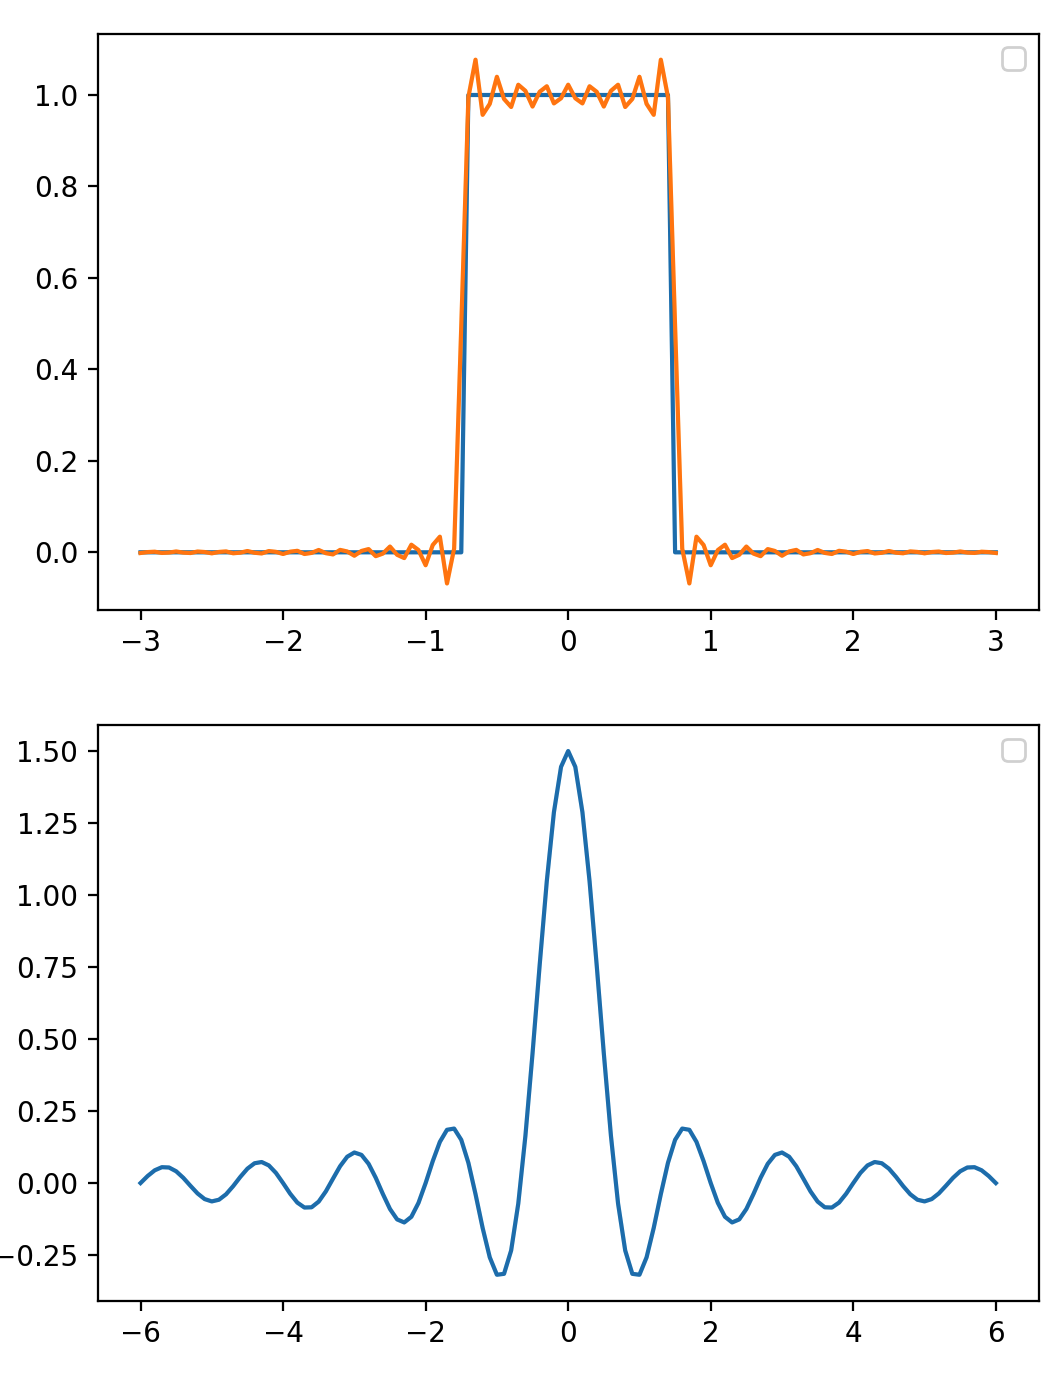
\includegraphics[width=\textwidth]{code/fourier_trafo.png}
    \end{minipage}
    \codecaption{dsv/code/fourier_trafo.py}{Berechnung und Darstellung von \eqref{eq:fourier:fourier_trafo}}\label{py:fourier_trafo}
\end{listing}

In \Cref{py:fourier_trafo} zeigen wir das Vorgehen zur Fourier-Analyse mittels numerischer Integration.
Es ist hier anzumerken, dass wir \q{nur} die Funktion \texttt{rect} definieren m"ussen und der Rest, also die Funktionen \texttt{kernel}, \texttt{analyse} und \texttt{synthese} unabh"angig hiervon sind.
Wir haben hier ein \namecref{py:fourier_trafo}, welches sich Methoden der Funktionalen Programmierung bedient.
Die Funktionen texttt{analyse} und \texttt{synthese} haben als Eingabewert die entweder die Funktion, oder die \acrlong{ft} einer Funktion.
Au"serdem liefern sie als Ausgabewert wieder \emph{Funktionen}, die wir einfach \q{aufrufen} k"onnen.
%
\subsection{Fourier-Transformation diskreter Signale}\label{sec:fourier:disc}
%
Wir n"ahern uns langsam der Fourier-Analyse von diskreten Signalen.
Schlie"slich wollen wir etwaige spektrale Analysen und dergleichen im Digitalen durchf"uhren, um die Vorz"uge von digitalen Rechenwerken dabei nutzen zu k"onnen.
Die vorher eingef"uhrten Transformationen sind zwar hilfreich f"ur theoretische Argumentation, wie beispielsweise beim Sampling-\Cref{stm:sampling_theorem}. 
Deshalb wenden wir uns nun der spektralen Analyse von diskreten Signalen zu.
Wir werden aber im Verlauf auch wieder "ahnliche Zusammenh"ange wie in \eqref{eq:fourier:c_k_fourier} finden.
%
\subsubsection{Fourier-Transformation diskreter periodischer Signale}\label{sec:fourier:disc_period}
%
Wir beginnen mit diskreten Signalen, die gleichzeitig periodisch sind, also ein $N$ existiert, sodass
\[
x[n] = x[n+kN] \Text{f"ur alle} n,k \in \Z 
\]
gilt.
Aus vorherigen Diskussionen in \Cref{sec:sampling} wissen wir einerseits, dass diskrete Signale ein periodisches Spektrum auf $(0,1)$ besitzen.
Andererseits wissen wir aus \Cref{sec:fourier:cont:period}, dass periodische Signale ein \emph{diskretes} Spektrum besitzen.
Wir finden also nun intuitiv, dass das Spektrum von diskreten periodischen Signalen \emph{ebenfalls} diskret und periodisch ist.
Denken wir zur"uck an \Cref{sec:sampling:disc_sin} so haben wir bereits alles Notwendige betrachtet.
Ein $N$-periodisches diskretes Signal ergibt sich aus der Linearkombination der diskreten Signale $x_k[\cdot] : \Z \rightarrow \C$ definiert durch
\[
x_k[n] = \exp\left(\jmath 2 \pi \frac k N n \right) \Text{mit} k = 0, \ldots, N-1.
\]
Das hei"st, f"ur $x[\cdot]$ setzen wir mit
\[
x[\cdot] = \Sum{k = 0}{N-1}{c[k] x_k[\cdot]}
\]
an.
Damit sind bereits beide Eigenschaften des Spektrums \q{eingepreist}.
Denn man erkennt in den $x_{k}[\cdot]$ die vorher erw"ahnte \emph{zweifache} Periodizit"at wieder, weil sowohl $x_{k+N}[\cdot] = x_{k}[\cdot]$ f"ur alle $k$ als auch $x_k[n+N] = x_k[n]$ f"ur alle $n$ gilt.

Es ist nun unser Ziel f"ur gegebene Werte $x[n]$ von $x[\cdot]$ die Werte des \emph{ebenfalls periodischen und diskreten} Signals $c[\cdot]$ zu bestimmen.
Dies verl"auft ganz analog zu \Cref{sec:fourier:cont:period}.
Wir definieren das Skalarprodukt $\ScPr{\cdot}{\cdot}$ f"ur $N$-periodische und diskrete Signale via
\[
\ScPr{x_1[\cdot]}{x_2[\cdot]} 
    = \Sum{n = 0}{N-1}{x_1[n] x_2[n]^\ast}.
\]
Das hei"st, dass wir periodisches Signal $x[\cdot]$ mit dem \emph{endlich-dimensionalen} Vektor $\bm x \in \C^{N}$ identifizieren, wir setzen also die Eintr"age des Vektors als $\bm x_i = x[i-1]$.
Dann k"onnen wir auch f"ur das entsprechende Skalarprodukt der Vektoren $\bm x_{1,2} \in \C^N$
\[
\ScPr{\bm x_1}{\bm x_2} 
    = \left(\bm x_2^\ast\right)^\trans \cdot \bm x_1 
    = \bm x_2^\herm \cdot \bm x_1
\]
schreiben.
Analog identifizieren wir die periodische und diskrete Sequenz $c[\cdot]$ mit dem Vektor $\bm c \in \C^N$.

Wie in \Cref{sec:fourier:cont:period} m"ussen wir nur 
\[
\ScPr{\bm x_k}{\bm x_\ell} 
    = \Sum{i=0}{N-1}{
        x_k[i] x_\ell[i]^\ast
    }
    = \Sum{i=0}{N-1}{
        \exp\left(\jmath 2 \pi \frac{i(k-l)}{N} \right)
    }
    = \begin{cases}
        N \Text{falls} k = \ell \\
        \frac{
            1 - \exp\left(\jmath 2 \pi \frac{(k-l)}{N} \right)^N   
        }{
            1 - \exp\left(\jmath 2 \pi \frac{(k-l)}{N} \right)
        } \Text{sonst}
    \end{cases}
    = \begin{cases}
        N \Text{falls} k = \ell \\
        0 \Text{sonst}
    \end{cases}
\]
berechnen.
Hierbei nutzen wir, dass $\exp(\jmath 2 \pi k) = 1$ f"ur alle $k \in \Z$.
Wie in \Cref{sec:fourier:cont:period} finden wir, dass also gilt $\ScPr{\bm x_k}{\bm x_\ell} = 0$, falls $k \neq \ell$ und $\ScPr{\bm x_k}{\bm x_k} = N$.
Damit ergibt sich bei Anwendung auf das eigentliche Signal $\bm x$ f"ur den Vektor $\bm c$, dass
\[
\ScPr{\bm x}{\bm x_\ell}
    = \ScPr{\Sum{k=1}{N}{\bm c_k \bm x_k}}{\bm x_\ell}
    = \Sum{k=1}{N}{\bm c_k \ScPr{\bm x_k}{\bm x_\ell}}
    = N \bm c_\ell
\Rightarrow
\bm c_\ell = \frac{1}{N}\ScPr{\bm x}{\bm x_\ell}.
\]
Zusammenfassend, kann man also sagen, dass sich folgende Analyse- und Synthesegleichungen ergeben:
\begin{equation}\label{eq:fourier:disc_analys_synth}
    x[n] = \Sum{k = 0}{N-1}{c[k]\exp(\jmath 2 \pi k n/N)}, \Text{und}
    c[k] = \frac{1}{N}\Sum{n = 0}{N-1}{x[n]\exp(-\jmath 2 \pi k n/N)}.
\end{equation}
In Vektorschreibweise l"asst sich der erste Teil durch
\begin{equation}\label{eq:fourier:disc_analys_synth_vec}
    \bm x = \Sum{k = 0}{N-1}{\ScPr{\bm x}{\bm x_k} \bm x_k}
\end{equation}
ausdr"ucken.

Weiterhin, k"onnen wir eine Matrix $\bm F_N \in \C^{N \times N}$ definieren, deren $k$-te Spalte den Vektor $\bm x_k$ beinhaltet.
Wir definieren also 
\[
\bm F_N = \left[
    \bm x_1, \ldots, \bm x_k, \ldots, \bm x_N 
\right]
\]
Dann k"onnen wir noch einen Schritt weitergehen und sehen, dass
\[
\bm c = \frac{1}{N} \bm F_N^\herm \bm x, \Text{und} \bm x = \bm F_N \bm c
\]
gilt.
Das hei"st, dass sich Fourier-Analyse und Fourier-Synthere von diskreten und periodischen Signalen durch eine Matrix-Vektor-Multiplikation durchf"uhren l"asst!
Das sind erst einmal gute Nachrichten, denn damit wissen wir, dass digitale Rechenwerke sehr gut darin sind, diese Transformation durchzuf"uhren.
Die hier vorgestellte Transformation nennen wir \gls{dft} und oft definiert man ein diskretes Signal $X[\cdot]$ durch
\begin{equation}
    X[k] = \frac{1}{N}\Sum{n = 0}{N-1}{x[n]\exp(-\jmath 2 \pi k n/N)} = c[k] = \bm c_k
\end{equation}
und nennt dieses dann die \gls{dft} von $x[\cdot]$.
Es ist anzumerken, dass der Vorfaktor $N^{-1}$ in manchen Lehrb"uchern oder Ver"offentlichungen auch bei der Synthese anstatt der Analyse auftaucht, oder aber \emph{beide} Gleichungen erhalten einen Faktor $N^{-1/2}$.

In \Cref{py:dft_1} zeigen wir ein einfaches Beispiel f"ur $x[\cdot] = u[\cdot] - u[\cdot-k]$.
Au"serdem zeigen wir auch die beiden Berechungsmethoden der $c[\cdot]$ -- einerseits mit der Definition und andererseits "uber ein Matrix-Vektor-Produkt.
%
\begin{listing}[ht]
    \noindent
    \begin{minipage}{0.51\textwidth}
        \strut\vspace*{-\baselineskip}\newline
        \inputminted[firstline=5, lastline=23]{python3}{code/dft_1.py}
    \end{minipage}%
    \begin{minipage}{0.48\textwidth}
        \strut\vspace*{-\baselineskip}\newline
        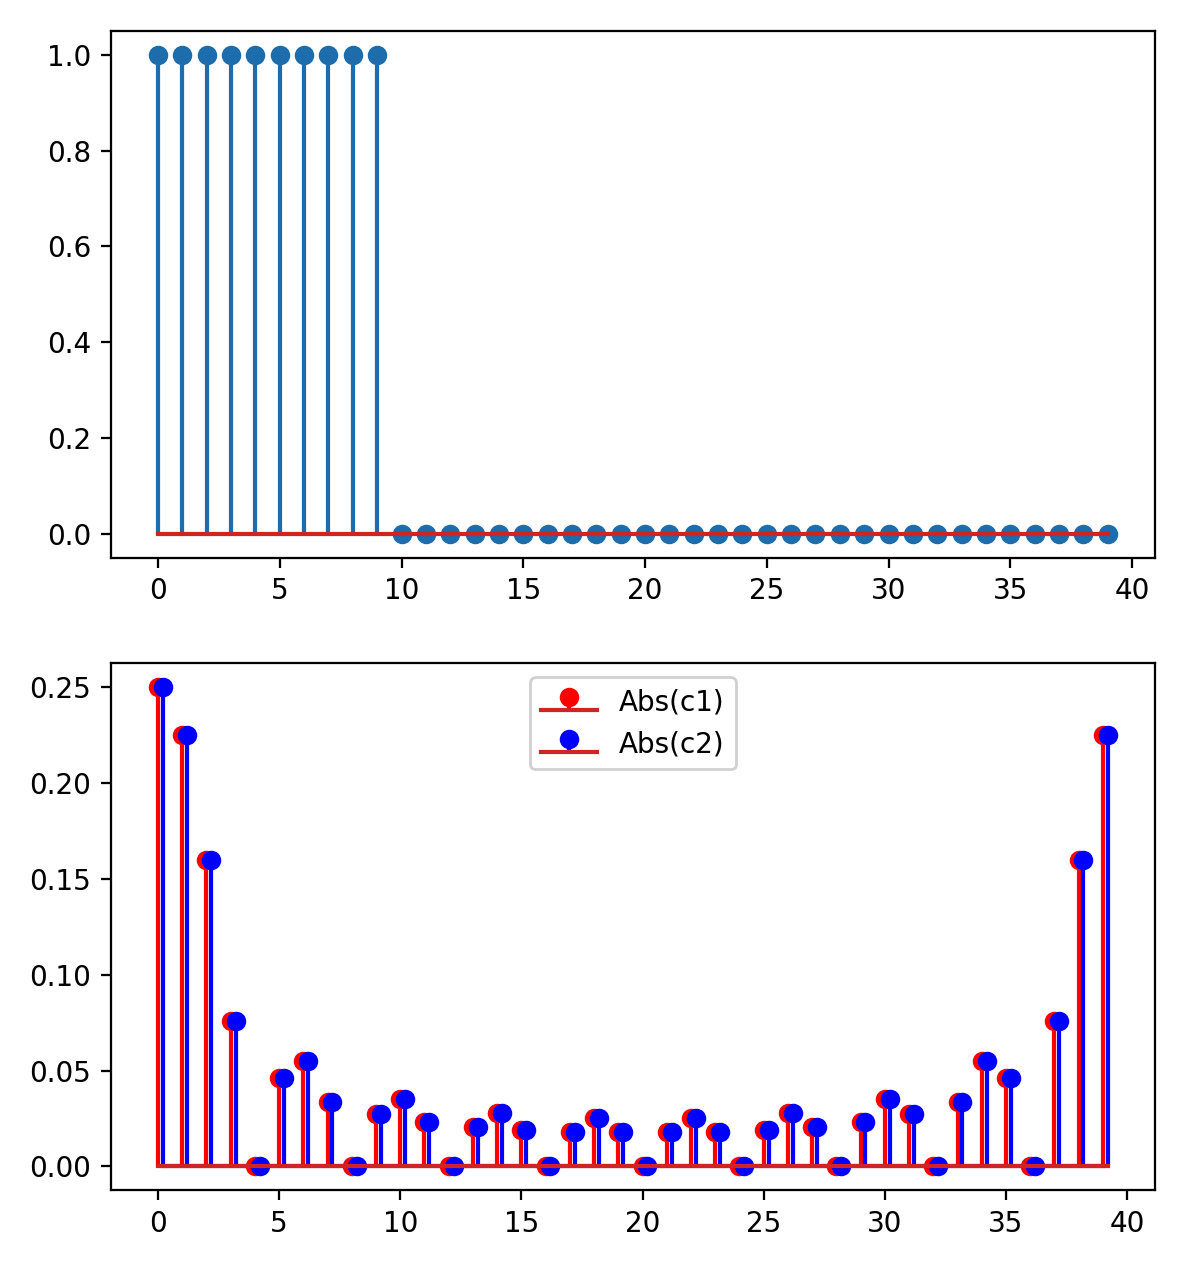
\includegraphics[width=\textwidth]{code/dft_1.png}
    \end{minipage}
    \codecaption{dsv/code/dft_1.py}{Berechnung und Darstellung von \eqref{eq:fourier:disc_analys_synth}}\label{py:dft_1}
\end{listing}
%
\subsubsection{Leichtungsdichte-Spektrum diskreter periodischer Signale}\label{sec:fourier:disc_period_power}
%
Da periodische Signale keine endliche Energie besitzen, betrachten wir die durchschnittliche Leistung "uber eine Periode.
Wir betrachten also f"ur ein $N$-periodisches Signal $x[\cdot]$ das Funktional
\begin{equation}
    P(x[\cdot]) = \frac{1}{N}\Sum{i=0}{N-1}{\Abs{x[n]}^2}.
\end{equation}
Dann k"onnen wir ganz analog zu vorher wieder herleiten, dass f"ur
\[
x[\cdot] = \Sum{i=0}{N-1}{c[k] x_k[\cdot]}
\]
und dessen Leistung gilt, dass
\[
P(x[\cdot]) = \Sum{i=0}{N-1}{\Abs{c[k]}^2}.
\]
Also auch hier finden wir wieder, dass sich die durchschnittliche Leistung einer Periode im Zeitbereich auf die Leistung einer Periode im Frequenzbereich "ubertr"agt.
Auch hier k"onnen wir die Folge $\Abs{c[\cdot]}^2$ als Leistungsdichte-Spektrum interpretieren.
\FloatBarrier
%
\subsubsection{Fourier-Transformation diskreter aperiodischer Signale}\label{sec:fourier:disc_aperiod}
%
Wiederum analog zu \Cref{sec:fourier:cont} ben"otigen wir noch eine Transformation f"ur diskrete Signale, die keine Periodizit"at aufweisen.
Hierzu definieren wir die zugeh"orige Fourier-Transformation, die wir \gls{dtft} nennen, durch
\begin{equation}\label{eq:fourier:dtft}
    X(f) = \Sum{n \in \Z}{}{x[n] \exp(-\jmath 2 \pi f n)},
\end{equation}
genau wie in \Cref{sec:sampling} bei der Herleitung von \eqref{stm:sampling_theorem}.
Im Unterschied zur \q{analogen} Fourier-Transformation \eqref{eq:fourier:fourier_trafo} sehen wir, dass $X$ nur f"ur Frequenzen $f \in (0,1]$ definiert ist, da das diskrete Signal $x_f[n] = \exp(\jmath 2 \pi f n)$ periodisch in $f$ ist.
Es gilt also $x_{f + k}[\cdot] = x_{f}[\cdot]$ f"ur alle $k \in \Z$.
Dies \q{passt} auch zur Natur von diskreten Signalen, da deren Frequenzbereich \emph{immer} periodisch sein muss.

Wir k"onnen nun f"ur die inverse Transformation \eqref{eq:fourier:dtft} mit \eqref{eq:fourier:fourier_series} vergleichen. 
Bis auf das Vorzeichen in der Funktion $\exp()$ gleicht \eqref{eq:fourier:dtft} einer Fourier-Reihe der periodischen Funktion $X$.
In der Tat, k"onnen wir die Folge $x[\cdot]$, also das urspr"ungliche Signal, als Fourier-Koeffizienten der \gls{dtft} $X$ durch
\begin{equation}\label{eq:fourier:idtft}
    x[n] = \Int{-1/2}{+1/2}{X(f)\exp(\jmath 2 \pi f n)}{f}
\end{equation}
wiederfinden.
Diese Synthese-Operation nennen wir dann \gls{idtft}.
Es ist wiederum anzumerken, dass die \gls{dtft} \q{nur} ein theoretisches Werkzeug ist, da sich im Allgemeinen die unendliche Summe in \eqref{eq:fourier:dtft} praktisch nicht realisieren l"asst, genauso wenig wie deren Resultat, eine kontinuierliche Funktion.

In \Cref{py:dtft} zeigen wir dennoch, wie man die \gls{dtft} einer aperiodischen Folge approximieren kann.
Wir studieren hierzu das Signal
\[
x[n] = \begin{cases}
    \frac{\omega}{\pi} \Text{f"ur} n = 0,\\
    \frac{\omega}{\pi} \frac{\sin(\omega n)}{\omega n} \Text{sonst}.
\end{cases}
\]
Dessen analytisch bestimmte \gls{dtft} $X$ ist
\[
X(f) = \Rect(f/(2 \pi \omega)),
\]
welche wir durch eine endliche Summe "uber die von uns verf"ugbaren Werte von $x[\cdot]$ bestimmen.

Nun treten hierbei mehrere Effekte zutage.
%
\begin{itemize}
\item Die Approximation der \gls{dtft} mittels des \q{abgeschnittenen} Signals $x$ stimmt noch nicht sehr gut mit der analytischen L"osung "uberein. 
Ver"andert man den Wert der Variable $N$ im Skript, tritt dieser Effekt st"arker oder schw"acher zutage.
\item Auch bei Erh"ohung von $N$ stellt sich immernoch keine Konvergenz von $X_{\rm approx}$ gegen $X_{\rm true}$ ein.
Dies liegt daran, dass die \gls{dtft} von $x[\cdot]$ nicht konvergiert, wie wir in \Cref{py:fourier_series} bereits gesehen hatten.
Diesen Effekt bezeichnet man allgemein als Gibbssches Ph"anomen\footnote{\url{https://en.wikipedia.org/wiki/Gibbs_phenomenon}}.
\item Augenscheinlich ist es besser die \gls{idtft} aus $X_{\rm approx}$ zu berechnen, als aus $X_{\rm true}$. Doch dies liegt legidlich daran, dass die numerische Integration der $\Rect$-Funktion nicht genau genug ist.
Erh"oht man die Anzahl der Punkte im Array \texttt{F}, dann stimmen im dritten Plot die drei Graphen besser "uberein.
\end{itemize}
%
\begin{listing}[ht]
    \noindent
    \begin{minipage}{0.51\textwidth}
        \strut\vspace*{-\baselineskip}\newline
        \inputminted[firstline=5, lastline=48]{python3}{code/dtft.py}
    \end{minipage}%
    \begin{minipage}{0.48\textwidth}
        \strut\vspace*{-\baselineskip}\newline
        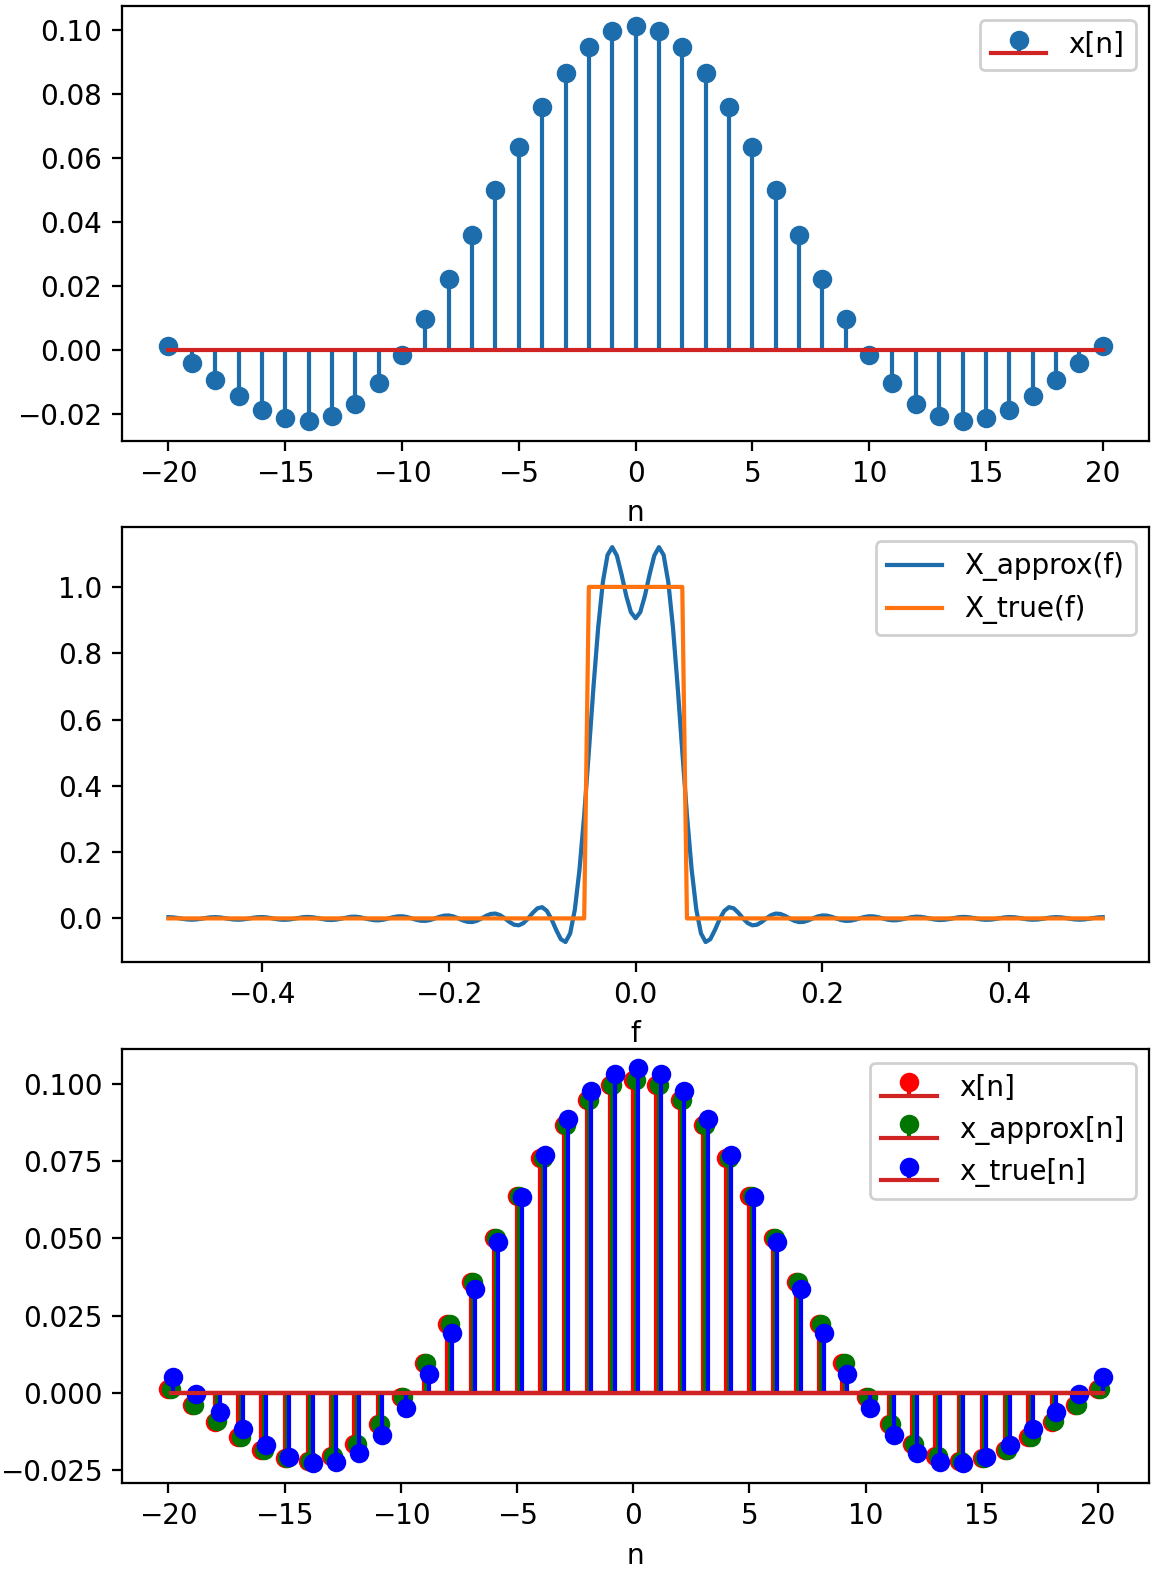
\includegraphics[width=\textwidth]{code/dtft.png}
    \end{minipage}
    \codecaption{dsv/code/dtft.py}{Berechnung und Darstellung von \eqref{eq:fourier:dtft}}\label{py:dtft}
\end{listing}
%
\FloatBarrier
\subsubsection{Leichtungsdichte-Spektrum diskreter aperiodischer Signale}\label{sec:fourier:disc_aperiod_power}
%
Die Energie eines diskreten Signals haben wir in \eqref{eq:disc_sig_energy} durch
\[
\mathcal{E}(x[\cdot]) = \Sum{n \in \Z}{}{\Abs{x[n]}^2} 
\]
definiert.
Wiederum k"onnen wir uns "uberlegen, dass dann f"ur die \gls{dtft} $X$ gilt, dass
\[
\mathcal{E}(x[\cdot]) = \Int{-1/2}{+1/2}{\Abs{X(f)}^2}{f}.
\]
Schlussendlich bezeichnet man dann
\[
S_{xx}(f) = \Abs{X(f)}^2
\]
als das Leichtungsdichte-Spektrum des Signals $x[\cdot]$.
In manchen Anwendungen ist es auch wieder sinnvoll Betrag und Phase von $X(f)$ zu analysieren.
%
\subsection{Eigenschaften der Fourier-Transformationen}\label{sec:fourier:proper}
%
Nachdem wir nun die notwendigen Definitionen gesammelt haben, wollen wir uns einige wichtige Eigenschaften der definierten Transformationen ansehen und eventuell auch f"ur \q{praktische} Dinge verwenden.
%
\subsubsection{Beziehung der Fourier-Transformationen und der \texorpdfstring{$z$}{z}-Transformation}
%
Wie wir in \cref{sec:ztrafo} gesehen haben, ist die $z$-Transformation f"ur ein diskretes Signal $x[\cdot]$ definiert durch
\[
X_{\z}(z) = \Sum{n \in \Z}{}{x[n]z^{-n}} \Text{mit \gls{roc}} r_2 < \Abs{z} < r_1.
\]
Wenn wir nun $z$ in Polarform $z = r \exp(\jmath 2 \pi f)$ ausdr"ucken und annehmen, dass $r_2 < r < r_1$, dann sehen wir, dass die $z$-Transformation von $x[\cdot]$ nichts anderes ist als die \gls{dtft} von $x[n] r^{-n}$ ist.
Mit anderen Worten ist die $z$-Transformation an einer Stelle $z=r \exp(\jmath 2 \pi f)$ die \gls{dtft} $X$ eines Signals gewichtet mit der Folge $w[n] = r^{-n}$ an der Stelle $f$.
Ist nun $1 \in \gls{roc}$ (und damit der gesamte Einheitskreis der komplexen Ebene), dann gilt
\begin{equation}\label{eq:fourier:ztrafo}
    X_{\z}(\exp(\jmath 2 \pi f)) = X(f)
\end{equation}
Wir haben uns zwar bis jetzt wenig Gedanken "uber die Existenz der Fourier-Transformation gemacht, doch hier finden wir einen Hinweis. 
Die \gls{dtft} existiert, beziehungsweise \emph{konvergiert}, falls $1 \in \gls{roc}$.
Da die \q{Form} der \gls{roc} immer kreisf"ormig ist, ist die gleichbedeutend mit der Tatsache, dass sich der Einheitskreis der komplexen Ebene in der \gls{roc} befindet.
Au"serdem kann man auch eine Fourier-Analyse von \gls{lti}-Systemen betreiben. 
Dann ist die \gls{bibo}-Stabilit"at von einem solchen System "aquivalent zur Tatsache, dass der Einheitskreis in der \gls{roc} liegt.
Wie wir gerade gesehen haben, folgt dann auch, dass \gls{bibo}-Stabilit"at ebenfalls durch die \emph{Existenz} der \gls{dtft} charakterisiert wird.
%
\begin{listing}[ht]
    \noindent
    \begin{minipage}{0.51\textwidth}
        \strut\vspace*{-\baselineskip}\newline
        \inputminted[firstline=5, lastline=46]{python3}{code/dtft_z.py}
    \end{minipage}%
    \begin{minipage}{0.48\textwidth}
        \strut\vspace*{-\baselineskip}\newline
        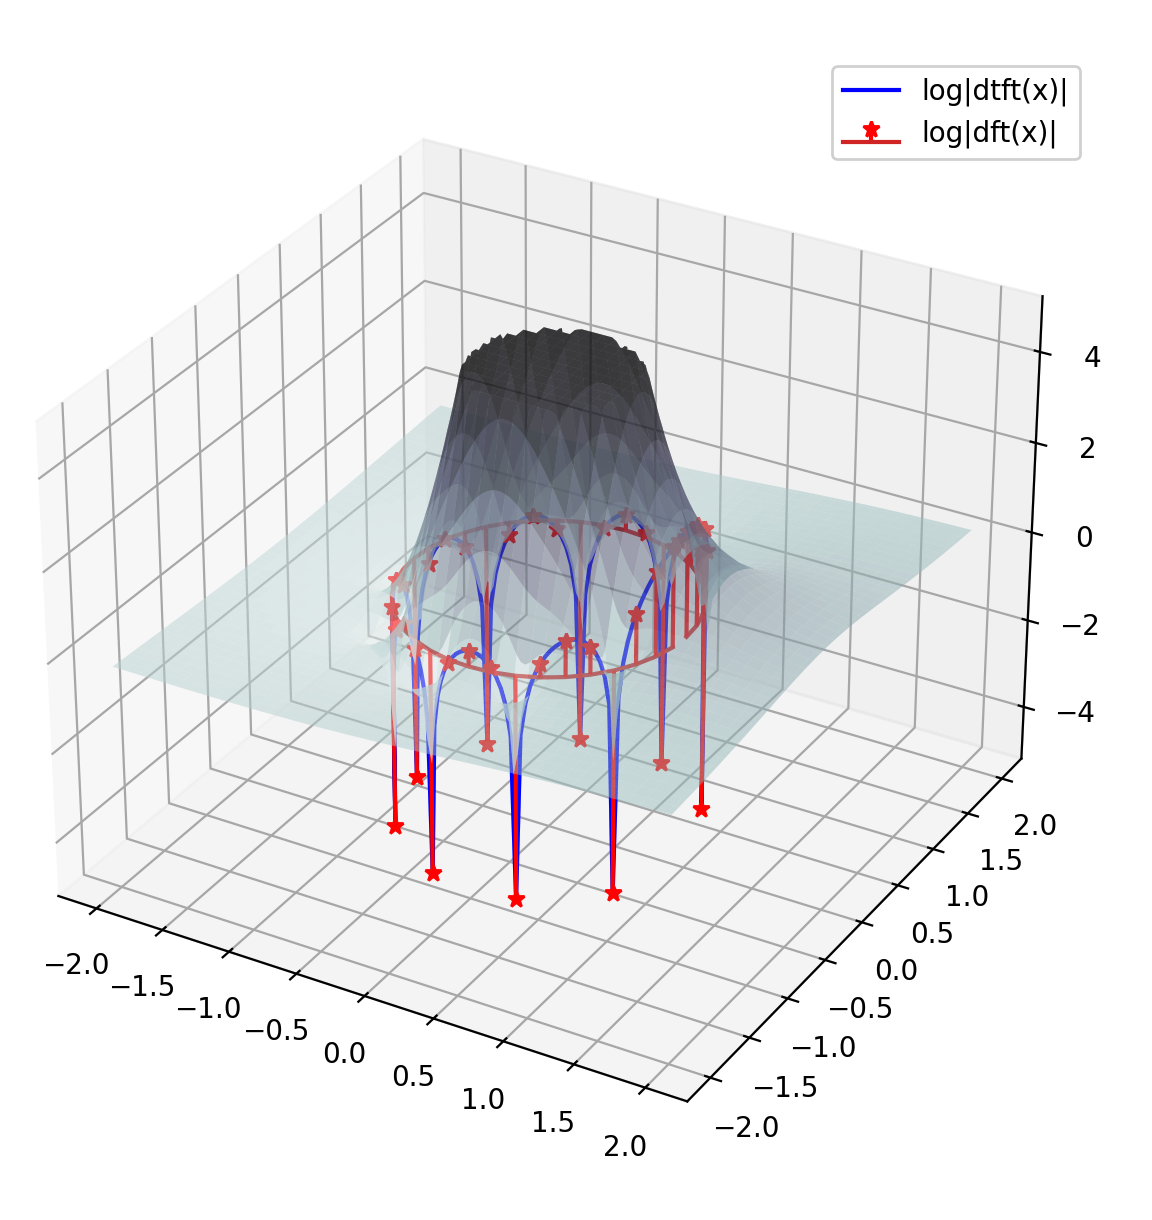
\includegraphics[width=\textwidth]{code/dtft_z.png}
    \end{minipage}
    \codecaption{dsv/code/dtft_z.py}{Berechnung und Darstellung von \eqref{eq:fourier:ztrafo}}\label{py:dtft_z}
\end{listing}

In \Cref{py:dtft_z} zeigen wir diesen Zusammenhang f"ur das gleiche Signal, wie in \Cref{py:dft_1}, interpretieren es hier aber einmal als aperiodisches Signal bei der Berechnung der \gls{dtft} und als periodisches Signal f"ur die Berechung der \gls{dft}.
Wir wissen aus den Eigenschaften der $z$-Transformation, dass das Signal $x[n] = u[n] - u[n-k]$ im $z$-Bereich einen $k$-fachen Pol bei $z = 0$ hat und $k-1$ Nullstellen auf dem Einheitskreis.

Wir k"onnen in dem Plot von \Cref{py:dtft_z} direkt sehen, dass die \gls{dtft} auf dem Einheitskreis in der Tat mit der $z$-Transformation "ubereinstimmt.
Au"serdem sehen wir gut den Pol bei $z=0$ und die $9$ Nullstellen auf dem Einheitskreis.
In den Plots der \gls{dtft} und der \gls{dft} sehen wir auch, dass sich die \gls{dft} durch Auswertung der \gls{dtft} ergibt.
Wir hatten vorher in \Cref{eq:fourier:c_k_fourier} schon gesehen, dass sich die Fourier-Koeffizienten $c[k]$ eines periodischen kontinuierlichen Signals aus der Auswertung der Fourier-Transformation an den richtigen Stellen ergeben.
Denselben Zusammenhang finden wir hier wieder, denn zwischen der \gls{dft} und der \gls{dtft} besteht derselbe Zusammenhang.
%
\FloatBarrier
\subsubsection{Weitere Eigenschaften der \texorpdfstring{\acrshort*{dft}}{DFT}}
%
Wir wollen analysieren, welche Eigenschaften die Beziehung zwischen einem diskreten $N$-periodischen Signal $x[\cdot]$ und und dessen \gls{dft} $X[\cdot]$ besitzt.

F"ur die meisten Eigenschaften macht es Sinn die \gls{dft} eines Signals der L"ange $N$ und die entsprechende \gls{idft} zu definieren durch
\begin{equation}\label{eq:fourier:dft_idft}
    X[k] = \Sum{n=0}{N-1}{x[n] W_N^{k \cdot n}}
    \Text{und}
    x[n] = \frac{1}{N}\Sum{k=0}{N-1}{X[k] W_N^{-k \cdot n}},
\end{equation}
wobei wir hier 
\begin{equation}\label{eq:fourier:weights}
    W_N = \exp(-\jmath 2 \pi / N)
\end{equation} 
definiert haben.
%
%
\paragraph{\gls{dft} ist periodisch:} Wir wissen bereits aus der Definition und den Eigenschaften von komplexen diskreten Harmonischen, dass
\[
X[k + \ell \cdot N] = X[k]
\]
f"ur alle $\ell \in \Z$ gilt.
%
%
\paragraph{"Ubereinstimmung mit \gls{dtft}:} Aus \Cref{py:dtft_z} wissen wir, dass
\[
X(k/N) = X[k]
\]
gilt -- wir die Werte der \gls{dft} also aus Auswertung der \gls{dtft} von $x[\cdot]$ erhalten.
Es ist wichtig zu erw"ahnen, dass die Frequenzen an denen die \gls{dtft} $X$ ausgewertet wird harmonische \q{Verwandte} sind, da wir $X$ an den Stellen $f = k/N$ auswerten.
%
%
\paragraph{Abgetastete Signale}\label{par:fourier:sampled_sig}
%
Ist $x[\cdot]$ aus Abtastung eines analogen Signals $x: \R \rightarrow \C$ entstanden, so erh"alt die Einheit von $f$ bei der \gls{dtft} eine Bedeutung, da dann \q{Perioden pro Sample} eine physikalische Interpretation zul"asst.
Tasten wir $x$ mit Sampling-Rate $F_s$ ab, so ist der Abstand zwischen zwei Samples in $x[\cdot]$ genau $1/F_s$.
Demzufolge erh"alt die \gls{dtft} $X(f)$ die Interpretation, dass wir das periodifizierte Spektrum von $x$ an den Stellen $f \cdot F_s$ betrachten.
Das hei"st beispielsweise bei einer Sample-Rate von \SI{44}{\kilo\hertz} entspricht der Bereich $f \in [-1/2,+1/2]$ dem \emph{physikalischen} Frequenzbereich von $F \in [\SI{0}{\hertz},\SI{44}{\kilo\hertz}]$.
Es ist jedoch zu beachten, dass wir bei der Betrachung der \gls{dtft} \emph{immer} nur das periodifizierte Spektrum erhalten. 
Das hei"st also, nur wenn wir Aliasing-frei abgetastet haben, also $F_s$ gro"s genug gew"ahlt haben, k"onnen wir aufschlussreiche Aussagen "uber das Spektrum von $x$ basierend auf der \gls{dtft} von $x[\cdot]$ treffen.
Wie bereits erw"ahnt, ergibt dann die \gls{dft} des Signals $x[\cdot]$ eben die periodifizierten spektralen Informationen von $x$ an den diskreten Frequenzen $k F_s/N$.
%
%
\paragraph{Reelle Signale}
%
Intuitiv sind reelle Signale \q{einfacher} als komplexe Signale. 
Deshalb mag es nicht verwunderlich sein, dass die \gls{dft} von reellen Signalen Struktur hat, in dem Sinne, dass wir einige Koeffizienten aus anderen schnell berechnen k"onnen.
Ist ein Signal reell, so gilt $x[n] = x[n]^\ast$ f"ur alle $n$.
F"ur $W_N$ gilt 
\[
W_N^\ell = \left(W_N^{-\ell}\right)^\ast
\Text{und}
W_N^{N-\ell} = \left(W_N^{\ell}\right)^\ast
\]
also gilt
\[
X[N-k] 
    = \Sum{n=0}{N-1}{x[n] W_N^{(N - k) n}}
    = \Sum{n=0}{N-1}{x[n]^\ast \left(W_N^{k n}\right)^\ast}
    = \Sum{n=0}{N-1}{x[n]^\ast W_N^{-k n}}
    = \left(\Sum{n=0}{N-1}{x[n] W_N^{k n}}\right)^\ast
    = X[k]^\ast
    = X[-k].
\]
Das hei"st, dass die \gls{dft} von rellen Signalen \q{konjugiert symmetrisch} um $k=0$ sind.
Dies hat zur Folge, dass man nur die Koeffizienten von $k=0$ bis $k = \lceil N/2 \rceil$ berechnen und speicher muss, was den Rechenaufwand halbiert.
Au"serdem wird hierdurch auch die \gls{idft} weniger komplex.
In Python ist es in solchen F"allen deshalb ratsam auf \mintinline{python}|np.fft.rfft| und \mintinline{python}|np.fft.irfft| zur"uckzugreifen.
Es sei noch angemerkt, dass sich noch viele weitere Redundanzen und Symmetrien ausnutzen lassen.
Siehe hierzu \cite[Kap. 7.2.1]{proakis2013}.
%
%
\paragraph{DC-Komponente und Nyquist-Sequenz}
%
Der Wert $X[0]$ wird oft als DC-Komponente, also Gleichanteil, bezeichnet, weil $W_N^0 = 1$, also ergibt sich speziell f"ur $X[0]$, dass
\[
X[0] = \Sum{n = 0}{N-1}{x[n]},
\]
was eben dem um Faktor $N$ skalierten Mittelwert des Signals $x[\cdot]$ entspricht.
Eine andere Interpretation ergibt sich aus der Betrachtung der \gls{dft} als Skalarprodukt, wobei wir die \q{"Ahnlichkeit} von $x[\cdot]$ mit der konstanten Sequenz $x_0[\cdot] = 1$ berechnet haben.
Ist ein Signal reell, so ergibt sich aus der Symmetrie des Spektrums, dass der DC-Anteil immer ebenfalls reell sein muss.
Gl"uck gehabt!

Der andere Extremfall tritt auf, wenn $k=N/2$. Hierbei wird vorausgesetzt, dass $N$ eine gerade Zahl ist.
Dann nennt man $x_{N/2}$ die Nyquist-Sequenz, denn wie wir in \nameref{par:fourier:sampled_sig} gesehen haben, entspricht $k=N/2$ der physikalischen Frequenz $F = (N/2) F_s / N = F_s/2$, also genau der \emph{maximalen} Frequenz, die ein Signal beinhalten darf, sodass es noch mit der gew"ahlten Sampling-Rate ohne Aliasing beobachtbar ist.
%
\begin{listing}[ht]
    \noindent
    \begin{minipage}{0.51\textwidth}
        \strut\vspace*{-\baselineskip}\newline
        \inputminted[firstline=4, lastline=46]{python3}{code/nyquist_seq.py}
    \end{minipage}%
    \begin{minipage}{0.48\textwidth}
        \strut\vspace*{-\baselineskip}\newline
        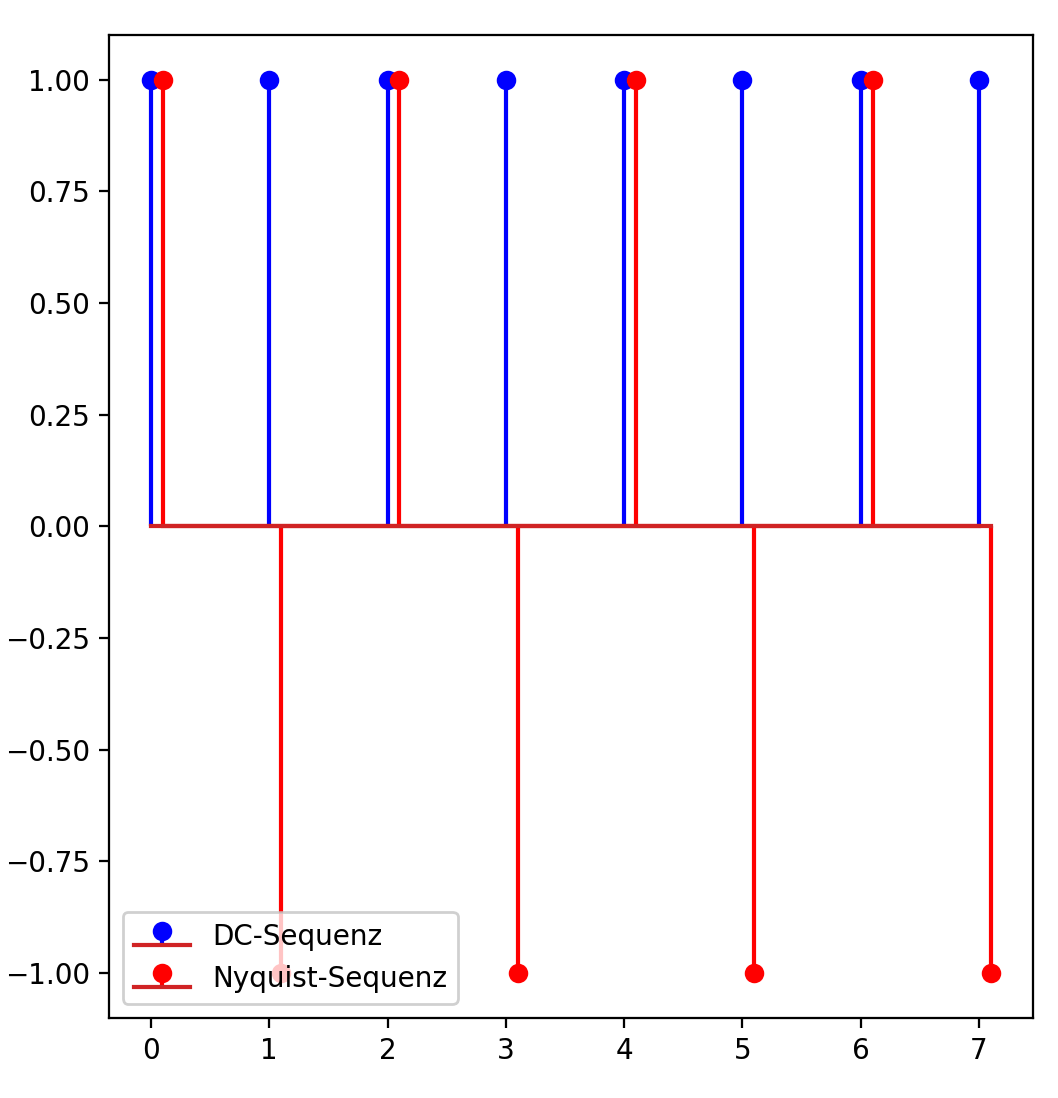
\includegraphics[width=\textwidth]{code/nyquist_seq.png}
    \end{minipage}
    \codecaption{dsv/code/nyquist_seq.py}{Darstellung der DC-Sequenz und der Nyquist-Sequenz f"ur $N=8$}\label{py:nyquist_seq}
\end{listing}

Man sieht in \Cref{py:nyquist_seq} gut, dass die beiden Sequenzen wirklich \q{Gegens"atze} darstellen, da $x_0[\cdot]$ die Anteile mit \q{minimaler} Variation/Frequenz aufsammelt, w"ahrend die Werte von $x_{N/2}[\cdot]$ genau so liegen, dass ein analoges Signal (und dessen Aliase), siehe \Cref{py:aliasing}, genau Frequenz $F_s/2$ (und Amplitude $1$) besitzen muss, um $x_{N/2}[\cdot]$ als Abtastwerte zu erhalten.
%
%
\paragraph{Zyklische Faltung im Zeitbereich}\label{par:fourier:cycl_conv}
%
Kommen wir nun zur wahrscheinlich wichtigsten Eigenschaft der \gls{dft} und dem Grund, warum digitale Signalverarbeitung "uberhaupt erm"oglicht wurde.
Wir haben bereits gesehen, dass \gls{lti}-Systeme durch eine Faltung realisiert werden k"onnen.
Gegeben zwei $N$-periodische Signale $x_{1,2}[\cdot]$ und betrachten wir deren \emph{zyklische} Faltung $\circledast$ definiert durch
\begin{equation}\label{eq:fourier:cyclic_conv}
x_3[m] = \Sum{n=0}{N-1}{x_1[n] \cdot x_2[(m-n) \mod N]} = (x_1 \circledast x_2)[m],
\end{equation}
dann kann man zeigen, dass
\[
X_3[k] = X_1[k] \cdot X_2[k]
\]
gilt.
Das hei"st, dass die zyklische Faltung von zwei periodischen Signalen wieder ein periodisches Signal ergibt, dessen \gls{dft} das Produkt der \glspl{dft} der gefalteten Signale ist.
Wenn wir an \gls{lti}-Systeme denken und uns erinnern, dass viele Filter als \gls{lti}-Systeme aufgefasst werden k"onnen, so ist klar, warum diese Eigenschaft wichtig ist.
Die digitalen Filter k"onnen also im Frequenzbereich sehr einfach angewendet werden, weil dort nur eine einfache punktweise Multiplikation notwendig ist.
Doch dies allein ist nicht ausreichend, denn wir ben"otigen noch einen effizienten weg, um zwischen Zeit- und Freqeunzbereich wechseln zu k"onnen.
Dies wird uns durch die \gls{fft} erm"oglicht werden.
In \Cref{py:dft_1} hatten wir bereits erfahren, dass man die \gls{dft} als Matrix-Vektor-Produkt formulieren kann, wozu etwa \glspl{flop} in der Gr"o"senordnung $N^2$ notwendig sind.
Die \gls{fft} erlaubt es aber eine \gls{dft} mit \glspl{flop} in der Gr"o"senordnung von nur $N \log{N}$ durchzuf"uhren.

Dann bel"auft sich eine effiziente Implementierung eines \gls{fir} Filters mit Impulsantwort $h[\cdot]$ auf folgende Schritte:
\begin{enumerate}
    \item Transformiere $x[\cdot]$ und $h[\cdot]$ in den Zeitbereich
    \item Punktweise Multiplikation von $Y[\cdot] = X[\cdot] \cdot H[\cdot]$ (NICHT die $z$-Transformation $H_{\z}$)
    \item R"ucktransformation von $Y[\cdot]$ zu $y[\cdot]$.
\end{enumerate}
%
Dieser Prozess wurde in \Cref{py:dft_conv} nachgestellt und wird mit der zyklischen Faltung im Zeitbereich verglichen.
Als Beispiel nehmen wir hier eine abgetastete Sinusfunktion, deren Werte mit Rauschen belegt sind.
Um das Signal ein wenig vom Rauschen zu befreien, implementieren wir ein gleitendes Mittel, siehe \Cref{py:moving_average}, dessen Mittelungsdauer wir mit einem \q{cut-off} einstellen k"onnen.
Wie man sieht, ist das Ergbenis der Faltung im Zeitbreich mit dem im Frequenzbereich identisch ist.
Au"serdem stellt sich durch die Mittelung eine Gl"attung der Werte ein, die mehr dem Verlauf des urspr"unglichen Signals "ahnelt.
Jedoch sieht man auch, dass sich die Phase des Resultates sich von der des Eingangs unterscheidet.
Diese Phase wird vom Filter $h$ aufgepr"agt und ist somit eine Konsequenz der gew"ahlten Signalverabeitung.
Es gibt M"oglichkeiten diesen Einfluss zu reduzieren, die aber "uber unser aktuelles Interesse hinausgehen.

Es sei hier angemerkt, dass dies er einfachste Fall ist, den man sich f"ur die sogenannte schnelle Faltung vorstellen kann.
Es ist beispielsweise nicht direkt klar, was zu tun ist, wenn $x[\cdot]$ und $h[\cdot]$ nicht diesselbe L"ange haben, was dazu f"uhrt, dass die resultierenden \glspl{dft} ebensfalls von verschiedener L"ange sind.
Dar"uber hinaus ist unsere Implementierung eine \q{offline}-Version in dem Sinne, dass die zu verarbeitenden Daten bereits im Speicher liegen.
Doch, wenn man an Echtzeitanwendungen, beispielsweise im Audiobereich, denkt so wird es notwendig sein, diese Operation auf Daten anzuwenden, die nicht vollst"andig im Zugriff liegen.
Au"serdem will man nat"urlich nicht immer eine zyklische Faltung, sondern eine \q{normale} Faltung implementieren.

Alle diese Probleme k"onnen aber mit einigen Tricks so umformuliert werden, dass man am Ende wieder eine zyklische Faltung rechnen kann.
Oft m"ussen hierzu das Signal order die Impulsantwort zielf"uhrend manipuliert werden, oder das Ergebnis nach Faltung noch prozessiert werden.

\begin{listing}[ht]
    \noindent
    \begin{minipage}{0.51\textwidth}
        \strut\vspace*{-\baselineskip}\newline
        \inputminted[firstline=4, lastline=18]{python3}{code/dft_conv.py}
    \end{minipage}%
    \begin{minipage}{0.48\textwidth}
        \strut\vspace*{-\baselineskip}\newline
        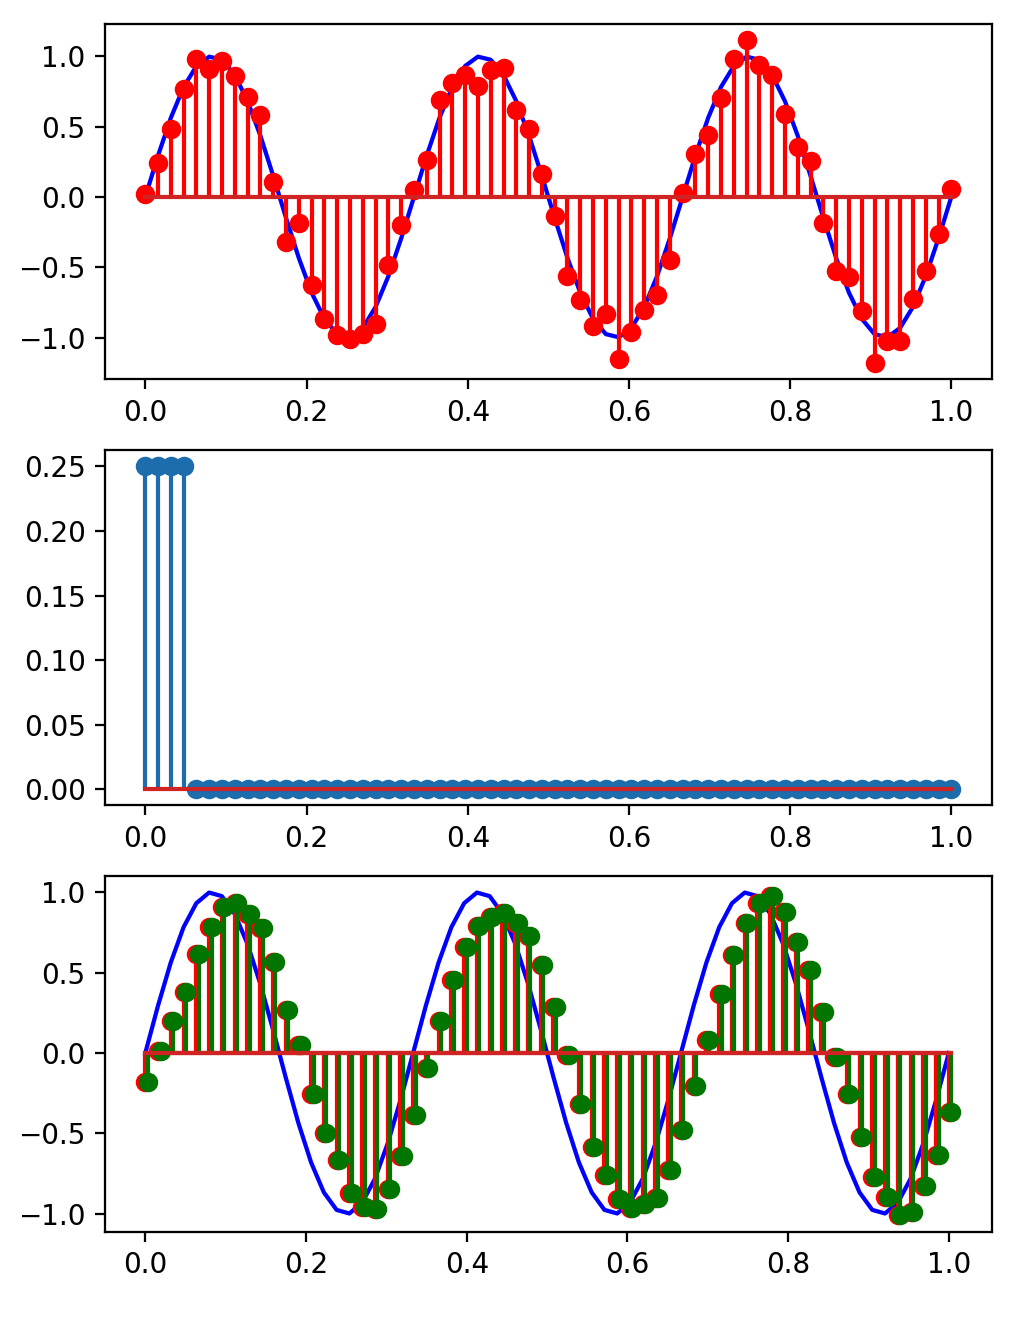
\includegraphics[width=\textwidth]{code/dft_conv.png}
    \end{minipage}
    \codecaption{dsv/code/dft_conv.py}{Zyklische/periodische Faltung im Zeitbereich und im Frequenzbereich.}\label{py:dft_conv}
\end{listing}
%
\paragraph{Zyklische Faltung im Frequenzbereich}
%
Als Dual zu \nameref{par:fourier:cycl_conv} gilt auch, dass die zyklische Faltung im Frequenzbereich eine Multiplikation der jeweiligen Signale im Zeitbereich zur Folge hat.
Es gilt also, f"ur ein Signal $x_3[\cdot]$ mit
\[
    x_3[n] = x_1[n] \cdot x_2[n],
\]
dass
\begin{equation}\label{eq:fourier:cycl_conv_dual}
    X_3[k] = \frac{1}{N}(X_1 \circledast X_2)[k].
\end{equation}
%
% \begin{itemize}
%     \item dft als approximation der dtft
%     \begin{itemize}
%         \item $s(t) = \exp(-t/\tau) \cdot \sin(\omega_0 \cdot t)$, 
%         \item $s(t) = \exp(-(t - \mu)^2/\sigma^2)$ (Uebung)
%     \end{itemize}
% \end{itemize}
